\documentclass[12pt,a4paper,]{article}
\usepackage{lmodern}
\usepackage{amssymb,amsmath}
\usepackage{ifxetex,ifluatex}
\usepackage{fixltx2e} % provides \textsubscript
\ifnum 0\ifxetex 1\fi\ifluatex 1\fi=0 % if pdftex
  \usepackage[T1]{fontenc}
  \usepackage[utf8]{inputenc}
\else % if luatex or xelatex
  \ifxetex
    \usepackage{mathspec}
    \usepackage{xltxtra,xunicode}
  \else
    \usepackage{fontspec}
  \fi
  \defaultfontfeatures{Mapping=tex-text,Scale=MatchLowercase}
  \newcommand{\euro}{€}
\fi
% use upquote if available, for straight quotes in verbatim environments
\IfFileExists{upquote.sty}{\usepackage{upquote}}{}
% use microtype if available
\IfFileExists{microtype.sty}{\usepackage{microtype}}{}
\ifxetex
  \usepackage[setpagesize=false, % page size defined by xetex
              unicode=false, % unicode breaks when used with xetex
              xetex]{hyperref}
\else
  \usepackage[unicode=true]{hyperref}
\fi
\hypersetup{breaklinks=true,
            bookmarks=true,
            pdfauthor={},
            pdftitle={},
            colorlinks=true,
            citecolor=blue,
            urlcolor=blue,
            linkcolor=magenta,
            pdfborder={0 0 0}}
\urlstyle{same}  % don't use monospace font for urls
\setlength{\parindent}{0pt}
\setlength{\parskip}{6pt plus 2pt minus 1pt}
\setlength{\emergencystretch}{3em}  % prevent overfull lines
\setcounter{secnumdepth}{0}

% Set margins
\usepackage[top=2.5cm,bottom=2.5cm,left=2.5cm,right=2.5cm]{geometry}
%\usepackage[T1]{fontenc}
\usepackage{fontspec}
%\fontspec{Minion Pro}
\setmainfont{Minion Pro}
\setromanfont[Numbers=OldStyle,Mapping=tex-text]{Minion Pro}
\DeclareTextCommand{\nobreakspace}{T1}{\leavevmode\nobreak\ }
%\usepackage[latin1]{iputenc}

\usepackage[spanish, es-tabla]{babel}
\usepackage{textcomp}
\usepackage{graphicx}
\graphicspath{{gfx/}} 
\usepackage{fancyhdr}
\usepackage{mathspec}
\usepackage{amsmath,amsthm}
\usepackage{xltxtra}
\usepackage{tabularx}
\usepackage{multirow}
\usepackage{tikz}
\usepackage{pgfplots}
\pagestyle{plain}

% Set figure legends and captions to be smaller sized sans serif font
\usepackage[font={footnotesize,sf}]{caption}

%\usepackage{siunitx}

% Adjust spacing between lines to 1.5
\usepackage{setspace}
\onehalfspacing
\raggedbottom

% Set colour of links to black so that they don't show up when printed
\usepackage{hyperref}
\hypersetup{colorlinks=true, linkcolor=black}

% Tables
\usepackage{booktabs}
\usepackage{threeparttable}
\renewcommand{\TPTnoteSettings}{\small
        \setlength\leftmargin{1.8em}%
        \setlength\labelwidth{1em}%
        \setlength\labelsep{.1em}%
}%
\usepackage{array}
\newcolumntype{x}[1]{%
>{\centering\arraybackslash}m{#1}}%

\begin{document}

\begin{titlepage}
    \begin{center}
    
        %\vspace*{1cm}
        

\includegraphics[width=5cm]{unab}\\
\vspace{0.1cm}
Facultad de Ciencias Biológicas\\
Escuela de Ingeniería en Biotecnología

        \vspace*{1cm}
        
       \large{ \textbf{ \uppercase{Establecimiento de un modelo molecular de respuesta inmune en tejido branquial de} \emph{Oncorhynchus mykiss} \uppercase{alimentado con $\beta$-glucanos}}}
        
        \vspace{0.5cm}
        
        \vspace{1.5cm}
 
        Proyecto de tesis presentado como parte de los requisitos para obtener el grado de \\
        \large{\textsc{Magister en Biotecnología}}\\ 
        
        \vspace{3cm}        
         
        \textbf{Director de Tesis:} Dr. Luis Mercado Vianco\\
        \textbf{Institución:} Pontificia Universidad Católica de Valparaíso       
       
       \vspace{0.8cm}          
        
             
        \vspace{0.5cm}     
        
        
         \vspace{2cm}
         presentado por:\\
         \vspace{0.1cm}
         \textbf{Sebastián Rodrigo Sariego Benítez}\\
         \textbf{Viña del Mar, Chile}
         
       

        
        
        \vfill
  
        Julio, 2013
        
 
 
     \end{center}
    \thispagestyle{empty}
\end{titlepage}

\clearpage

\section{Introducción}\label{introducciuxf3n}

Las primeras truchas en Chile hacen su aparición a fines del siglo XIX,
específicamente en 1880, fue en este año cuando en la recién hace 5 años
fundada ciudad Lota, actual región del Bio-Bio se introdujeron las
primeras ovas de la llamada ``Trucha común'', actualmente conocida como
Trucha Fario (\emph{Salmo trutta}). No fue hasta en la primera década
del siglo XX que el gobierno de ésa época, respondiendo a las
inquietudes de un naturalista alemán llamado Federíco Albert, quien
había realizado un catastro de las posibles especies de salmónidos que
podrían ser introducidos en nuestro país, el cual reconoce el potencial
poder económico de estos salmónidos e introduce, junto a la creación de
la Piscicultura Río Blanco, tres especies traídas desde Francia, la
Trucha Fario, la Trucha arcoíris (\emph{Oncorhynchus mykiss}) y el
Salmón del atlántico (\emph{Salmo salar}).

\subsection{El género
\emph{Oncorhynchus}}\label{el-guxe9nero-oncorhynchus}

Onchorhyncus corresponde a uno de los 10 generos de la familia
Salmonidae y tiene alrededor de 12 especies, incluyendo \emph{O.mykiss}
(trucha arcoíris), \emph{O. nerka} (salmón rojo), \emph{O. gorbuscha}
(salmón rosado), \emph{O. tshawytscha} (salmón chinook), \emph{O.
kisutch} (salmón coho) , entre otros. Se distribuyen principal y
naturalmente por una vasta zona que comprende desde California hasta el
mar de Behring y el oceáno ártico (C. Groot et al., 1991).

Algunas características principales de este genero son las siguientes

\begin{itemize}
\itemsep1pt\parskip0pt\parsep0pt
\item
  Son peces anádromos, es decir emigran al mar cuando son juveniles y
  luego vuelven al agua dulce para reproducirse.
\item
  A su vez, en su mayoria solo se reproducen una vez, por lo tanto son
  semélparos.
\item
  Tienen baja tasa de fecundidad (2 a 5mil ovas) y grandes huevos
  (5-8mm)
\end{itemize}

En Chile encontramos la Trucha arcoíris, el Salmón coho
(\emph{Oncorhynchus kisutch}) y el Salmón chinook (\emph{Oncorhynchus
tshawytscha}) como representantes de este genero.

La trucha arcoiris, descrita inicialmente por Walbaum en 1972 tiene un
cuerpo alargado fusiforme con 60 a 66 vertebras, con 3 a 4 espinas
dorsales, 10 a 12 rayos dorsales blandos, 3 a 4 espinas anales, 8 a 12
rayos anales blandos y 19 rayos caudales. Presentan una aleta con gran
tejido adiposo, la cual usualmente contiene un borde negro. Tienen como
coloración principal tonalidades de azul a verde oliva, sobre una banda
rosa a lo largo de la linea lateral y plateada por debajo de ella,
configuración cromática que le da su nombre \emph{arcoíris}.

\begin{figure}[h!]
    \centering
    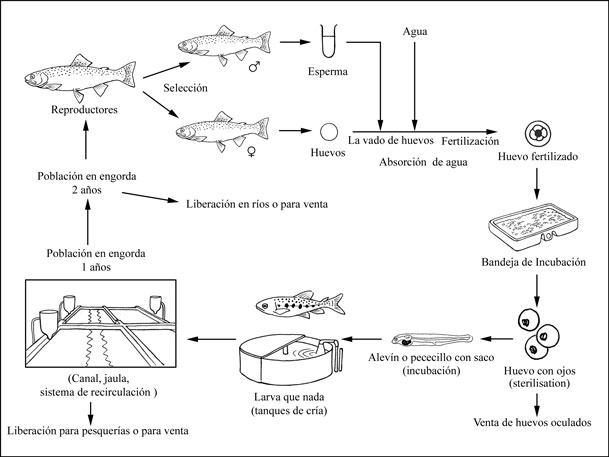
\includegraphics[width=9cm]{1} 
    \caption {Ciclo productivo de la trucha arcoíris}
    \label {fig:ciclo}
\end{figure}

Este pez es resistente, de crecimiento rápido y tolerante a una amplia
gama de manipulaciones y ambientes, pudiendo así ocupar una variedad de
hábitats y diferentes temperaturas. La temperatura ideal para el cultivo
de la trucha arcoíris está por debajo de 21º C, aunque en etapa de
desove y crecimiento la temperatura tiene que estar en el rango de 9 a
14ºC (Figura \ref{fig:ciclo}).

\subsubsection{Situación actual en
Chile}\label{situaciuxf3n-actual-en-chile}

Los desembarques de Trucha arcoíris han aumentado cercano al 1500\% en
20 años (Figura \ref{desembarques}), con una tasa de crecimiento
porcentual promedio del alrededor del 15\% (Sernapesca, 2012), en
términos monetarios, el año 2013 la exportación de este producto genero
ventas alrededor de los 300 millones de dólares, lo que lo convierte en
una de las 3 especies más cosechadas en Chile junto al Chorito y el
Salmón del atlántico (Subpesca, 2013).

\begin{figure}[h]
\begin{tikzpicture}
\begin{axis}[
axis lines*=left,
ybar,
scaled y ticks=false,
ylabel={Toneladas},
xlabel={Año},
xlabel absolute, xlabel style={yshift=-0.5cm},
ylabel absolute, ylabel style={yshift=0.5cm},
xtick={1992, 1993, 1994, ..., 2012},
  /pgf/number format/.cd,
        use comma,
        1000 sep={},
x tick label style={rotate=45,anchor=east},
yticklabel style={/pgf/number format/fixed},
width=14cm, height=7cm]
\pgfplotstableread[col sep=comma, header=has colnames]{datos/desembarques.csv}\loadedtable;

\addplot table[x=Año, y=Toneladas] {\loadedtable};
\end{axis}
\end{tikzpicture}
\caption{Desembarques de Trucha arcoíris en Chile} \label{desembarques}
\end{figure}

Uno de los principales aspectos a tener en cuenta con una especie con
tal valor comercial es su respuesta inmune. Gran parte de la mortalidad
de estas especies deriva de distintos tipos de infecciones, como por
ejemplo las provocadas por \emph{Flavobacterium psychrophilum} y
\emph{Piscirickettsia salmonis}, llegando a haber muertes en casos de
hasta el 50\% y 34\% de la producción respectivamente. La explicación de
esto radica en la pérdida del equilibrio ambiente-patógeno-hospedero, lo
cual genera las condiciones que hacen aumentar la enfermedad y
mortalidad en el cultivo. En el caso de la acuicultura (Industria que
representa cerca de un 50\% de la oferta mundial de pescado) (FAO,
2012), un grave problema son las enfermedades asociadas a cultivos
masivos de peces, mayoritariamente relacionadas al stress en que se ven
sometidos los organismos como también por el crecimiento acelerado de la
producción y los sistemas de cultivo actuales (FAO, 2012; Georgiadis et
al., 2001)⁠⁠. Estas enfermedades, cualquiera sea su origen, pueden tener
un alto impacto negativo en la producción mundial, lo que equivale a
grandes pérdidas económicas (Z. J. Shao, 2001)⁠. Por lo tanto es
necesario tener información del sistema inmune en peces, para así poder
minimizar los efectos producidos por estas enfermedades y en algunos
casos prevenirlos.

\subsection{Sistema inmune en peces}\label{sistema-inmune-en-peces}

La comprensión de la funcionalidad del sistema inmune de peces,
especialmente en teleósteos, al igual que en vertebrados superiores se
puede entender como una respuesta innata o inespecífica y una respuesta
adaptativa o especifica. La respuesta inmunológica presentada por los
peces está bien desarrollada e integrada, aunque si, influenciada
notoriamente por los cambios estacionales y la temperatura (Fernández et
al., 2002; Olabuenaga, 2000)

La respuesta inmune innata o inespecífica en peces es muy importante, ya
que constituye la primera y más importante línea de defensa del pez
frente a un gran número de patógenos, en esta respuesta convergen
factores humorales y celulares (Fernández et al., 2002; Olabuenaga,
2000; L.-Y. Zhu et al., 2012). Este tipo de inmunidad está basado en el
reconocimiento no clonal de los componentes estructurales o secretados
de los patógenos microbianos (Athman et al., 2004)⁠, los cuales son
llamados patrones moleculares asociados a patógenos (o PAMPs, por sus
siglas en inglés), estos a su vez son reconocidos por receptores de
reconocimiento de patrón (PRR, por sus siglas en inglés) (Gordon, 2002),
entre los cuales se encuentran receptores de tipo Toll (TLR, por sus
siglas en inglés), el receptor de complemento tipo-3 (CR3), Dectina-1,
proteína C-reactiva, entre otros (Rondon-Barragan, 2010). Entre los
PAMPs más clásicos se puede encontrar a las secuencias de ADN CpG sin
metilar, los lipopolisacáridos (LPS) y el RNA bicatenario viral. La
interacción entre los PRR (como los TLR) y los PAMP es la reacción que
desencadenará e iniciará la transducción de señales intracelular que
resultara en la expresión de genes involucrados en la inflamación,
respuesta antiviral y maduración de células con fenotipo dendrítico
(Aghaallaei et al., 2010)⁠; TLRs individuales activan factores de
transcripción únicos y comunes a través de diferentes vías de
señalización para generar una respuesta biológica especifica ante
microorganismos (N. C. Bols et al., 2001; A. E. Ellis, 2001; Kawai et
al., 2005)

Entre las células involucradas la fase celular inespecífica de la
respuesta inmune están las células citotóxicas no específicas (NCC, por
sus siglas en inglés), células fagocíticas, y granulocitos (Ainsworth,
1992; A. E. Ellis, 1977). Las células NCC en peces se encuentran
principalmente en el riñón cefálico, el bazo, sangre periférica y el
timo, son células citotóxicas inespecíficas, es decir ejercen su acción
en diferentes células diana sin un reconocimiento previo, las cuales
requieren un contacto célula-célula para poder efectuar la lisis celular
(Graves et al., 1984). Dentro de las células fagocíticas los neutrófilos
representan aproximadamente en promedio a un 11\% de los leucocitos en
sangre, son también llamados polimorfonucleares o leucocitos
específicos, su capacidad fagocítica es baja, ya que ingieren poco
material extraño, aunque poseen la mayoría de la batería enzimática para
este trabajo. Los eosinófilos y basófilos son los granulocitos con menor
presencia en peces, aunque en el caso de los eosinófilos se han logrado
encontrar en peritoneo u otros tejidos como el intestino, mientras que
los basófilos tienen escasa presencia en estos organismos (D. Palić et
al., 2011).

Dentro del sistema fagocítico mononuclear, podemos encontrar a los
monocitos y a los macrófagos (derivados de estas últimas), los primeros
son móviles y generalmente más grandes que los demás leucocitos, en el
caso de los macrófagos, pueden fagocitar partículas mucho más grandes,
son abundantes en el bazo y riñón cefálico, aunque también se han
encontrado en mucosa olfatoria (Castro et al., 2011; Olabuenaga, 2000).

Entre los componentes moleculares asociados a la respuesta innata del
sistema inmune de peces podemos encontrar a las citoquinas, las cuales
son una familia de proteínas de bajo peso molecular (comúnmente
glicosiladas) y secretadas por células del sistema inmune activadas
previamente frente a la exposición de diferentes componentes patógenos
(Salazar-Mather et al., 2006)⁠. Estas citoquinas pueden dividirse en
interferones (IFNs), interleuquinas (ILs), factores de necrosis
tumorales (TNFs, por sus siglas en inglés), factores estimuladores de
colonias y quimioquinas (Savan et al., 2006)⁠. Las interleuquinas son
citoquinas producidas principalmente por linfocitos T CD4+, aunque
también son secretadas por una gran variedad de tipos celulares, como
por ejemplo los macrófagos/monocitos y las células endoteliales (C. J.
Secombes et al., 2011), las quimioquinas, o también llamadas citoquinas
quimiotácticas (o quimioatractantes) son una familia de citoquinas que
son liberadas por la mayoría de tejidos infectados en los estadíos
tempranos de infección. Las citoquinas pueden dividirse en distintas
familias según sea la organización de sus cisteínas.

Dentro de la familia de las interleuquinas podemos encontrar la
Interleuquina 1$\beta$, la citoquina proinflamatoria mas estudiada, todo
debido a su rol mediador de enfermedades autoinflamatorias. Es producida
principalmente por macrófagos activados, celulas dendríticas y
monocitos, y afecta a casi cualquier tipo celular, jugando un rol
central en la generación de respuestas sistémicas y locales a la
infección, asi como también en respuesta a daños y desafíos
inmunológicos (Reis et al., 2012). Esta citoquina potencialmente induce
la proliferación, diferenciación y activación de celulas no específicas,
como NK, macrofagos, etc\ldots{}, así como también una respuesta inmune
específica, activando linfocitos B y T (Hong et al., 2004;
Taechavasonyoo et al., 2013). Junto con IL-1$\beta$ existe otro marcador
que sirve para evaluar si es que los inmunoestimulantes inducen o no una
respuesta inflamatoria, este otro marcador es el Factor de necrosis
tumoral (TNF$\alpha$). este factor tiene una variedad de funciones
inmunológicas, regulando la inflamación y la respuesta inmune
celular(Teles et al., 2011; T. Wang et al., 2004; J. Zou et al., 2003).
Promueve la necrósis hemorrágica de tumores, así como también mejora la
fagocitosis y citotoxicidad de neutrofilos. Mejora la sintesis de
prostaglandina E2 y oxido nítrico (NO), y modula la expresión de muchas
citoquinas, incluyendo IL-1, IL-6 y algunas quimioquinas. IL-1$\beta$ y
TNF$\alpha$ son ampliamente usados como marcadores de respuesta inmune
innata. (Z. Zhang et al., 2009)

Otra citoquina importante en el proceso inmunitario es Interferón Gamma
(IFN$\gamma$), perteneciente a la familia de los Interferones, moleculas
encargadas principalmente en la respuesta viral, aunque también son
importantes reguladores del sistema inmunitario innato y adaptativo
(Savan et al., 2006). El IFN-$\gamma$ es producido en una primera etapa
por celulas NK estimuladas por las interleuquinas 12 y 18, las cuales
son producidas por fagocitos mononucleares y celulas presentadoras de
antígenos (APCs, por sus siglas en inglés). Al ser secretada esta
molécula se une a su receptor y por la via Jak/STAT promueve la
activación de macrófagos aumentando la sintesis de la fagocito oxidasa
dependiente de NADPH (gp91\textsuperscript{phox} y
p67\textsuperscript{phox}), la oxido nítrico sintasa 2 (NOS2), p47
GTP-asa y la proteina de union a guanilato, así como también aumenta las
moleculas de MHC de clase 2 en macrofagos y otras APCs (U. Boehm et al.,
1997). Por lo tanto en contraste con los interferones de tipo I
(IFN-$\alpha$/$\beta$) el IFN$\gamma$ juega un rol clave en la
activación de macrofagos para aumentar destrucción de patógenos
bacterianos, protozoos y virales(Fields et al., 2007).

La interleuquina 12 (IL-12) es una citoquina heterodimérica, compuesta
por la subunidades P35 y P40, la primera miembro de la familia de la
interleuquina 6 con 4 $\alpha$-helices en su topología y p40 recuerda
una forma asociada a un receptor de citoquinas solubles(Huising et al.,
2006; Yoshiura et al., 2003). Esta citoquina pro-inflamatoria es
producida en las etapas iniciales de la respuesta inmune por monocitos,
macrófagos, celulas dendríticas y neutrofilos, y una de sus principales
funciones es inducir la sintesis de otras citoquinas, como el
anteriormente nombrado IFN-$\gamma$, que sirve como orquestador en la
maduración de un linfocito T \emph{naive} a un fenotipo Th1 (Nascimento
et al., 2007), y es gracias a esta función se considera como un
medidador entre la respuesta innata y adaptativa de la inmunidad(Lu
Zhang et al., 2014).

Dentro de las moleculas efectoras de la respuesta inmune la oxido
nítrico sintasa de tipo inducible (iNOS), propia de fagocitos (Wu et
al., 2008; Zhao et al., 2010), aumenta su expresión durante eventos de
inflamación, y a su vez, es propia del estallido respiratorio de los
macrófagos proveyendo así a la celula de un ambiente citotóxico ideal
para los eventos pro-inflamatorios por la producción de Oxido Nítrico
(NO), catalizando la oxídación de L-arginina (Yang et al., 2013). Esta
molecula, puede ser activada en monocitos, macrófagos, células
dendríticas, neutrofilos y células NK ya sea por citoquinas,
endotoxinas, o ambas (Bogdan, 2001; MacMicking et al., 1997). estas
características demuestran la importancia del rol de iNOS y su producto
gaseoso NO en el sistema inmune, ya que a diferencia de las otras NOS,
la neuronal (nNOS) y la endotelial (eNOS) esta no tiene una sintesis
basal ni constitutiva, haciendo de esta molecula un marcador
inmunológico de importancia para estudiar procesos inmunológicos.

Otras moléculas efectoras presentes en la respuesta innata frente a
patógenos son los péptidos anti-microbianos (AMP, por sus siglas en
inglés), moléculas con la capacidad de destruir y/o neutralizar
microorganismos patógenos directamente, son moléculas pequeñas,
anfipáticas y catiónicas (L. Mercado et al., 2005)⁠, y están ampliamente
extendidos por los reinos vegetal y animales (Zasloff, 2002). Los
mecanismos de acción anti-bacteriana de estos AMP pueden entenderse
desde dos puntos de vista diferentes: 1. La estructura anfipática puede
unirse selectivamente a la membrana bacteriana y generar poros
transmembrana, los cuales destruyen a la bacteria desintegrando la
membrana, y 2, los AMP pueden directamente entrar a la bacteria e
interactuar específicamente con factores de crecimiento y metabolismo
bacteriano eventualmente generando la muerte bacteriana (Wimley, 2010;
L.-Y. Zhu et al., 2012)⁠. Entre los péptidos anti microbianos descritos
en peces podemos encontrar cuatro grandes grupos, las defensinas,
proteínas de macrófagos asociadas a resistencia natural (Pramps, por sus
siglas en inglés), NK-lisina y hepcidinas.

Otra familia de péptidos antimicrobianos son las Catelicidinas,
presentes generalmente en neutrófilos y superficies de mucosas, su
actividad se centra principalmente en su interacción con la membrana
plasmática de la bacteria para eventualmente destruirla, fueron
primeramente descritas en mamíferos y luego se han encontrado en
distintos peces teleósteos, algunos casos son los de trucha arcoíris
(C.-i. Chang et al., 2005)⁠, bacalao (Maier et al., 2008), salmón del
atlántico (C.-I. Chang et al., 2006), entre otras.

Además de poseer una robusta y bien desarrollada respuesta inmune innata
como se explicaba anteriormente, los peces también cuentan con una
respuesta adaptativa, con componentes celulares y humorales
(Alvarez-Pellitero, 2008)⁠, en este último grupo se encuentran los
anticuerpos, los cuales son proteínas pertenecientes al grupo de las
inmunoglobulinas (Ig), en el caso de los peces producen inmunoglobulinas
del tipo M, T y D (Bengtén et al., 2002; Ling Zhang et al., 2011; L.-Y.
Zhu et al., 2012)⁠, siendo la primera la más importante, estando
presente en el suero, el mucus y la bilis. Los anticuerpos son
producidos por linfocitos B activados al reconocer algún antígeno, ya
sea en solución o presentado por alguna célula presentadora de antígeno,
que en el caso de los peces principalmente son macrófagos, y tienen
variadas funciones, pueden actuar como moléculas efectoras en el suero,
o también como receptores de superficie de linfocitos B.

Una de las principales diferencias entre el sistema inmune de peces
teleósteos con el de mamíferos es la carencia de medula ósea y ganglios
linfáticos, por lo cual no se puede marcar una diferencia entre órganos
hematopoyéticos y órganos linfoides (Fernández et al., 2002; Olabuenaga,
2000)⁠. Entre los principales órganos pertenecientes al sistema inmune
de peces podemos encontrar el timo, el riñón y el bazo. El riñón
cefálico es el principal órgano en la diferenciación de linfocitos B, ya
que es el primer órgano en el que aparecen estas células durante el
desarrollo del pez, también es el órgano donde se produce la
eritropoyesis, granulopoyesis, linfopoyesis y monocitopoyesis (Whyte,
2007), por lo que se le puede considerar a la vez un órgano análogo a la
medula ósea de los mamíferos (Razquin et al., 1990)⁠. Los centros
melanomacrofágicos son una agregación de macrófagos que contienen
melanina, un pigmento de color oscuro, su tamaño y número está
directamente relacionado con el estado del pez, ya que estas variables
aumentan considerablemente en peces enfermos, donde el catabolismo ha
sido excesivo. Algunos estudios ontogénicos realizados en salmónidos
sugieren que la función del bazo no es esencial en la maduración del
sistema inmunológico, ya que los linfocitos del timo y riñón cefálico
estarían más involucrados que este órgano en esta maduración. Otros
estudios sin embargo indican, que bajo un desafío antigénico aparecen
linfocitos B en el bazo, teniendo parámetros similares a los presentados
por estas células en otros órganos como el riñón cefálico.

\clearpage

\subsection{Inmunoestimulantes}\label{inmunoestimulantes}

Los inmunoestimulantes han sido descritos como componentes necesarios
para la acuicultura, ya que mejoran la respuesta innata y proveen
resistencia a patógenos. Diferentes de estas sustancias, como los
B-glucanos, productos bacterianos y constituyentes de las plantas pueden
iniciar directamente la activación de mecanismos de defensa innata
actuando en receptores y desencadenando la activación de distntos genes
que puedan resultar en la producción de moleculas antimicrobianas
(Bricknell et al., 2005; Kumari et al., 2006). A pesar de la evidencia
demostrada sobre el uso benéfico de estas sustancias como potenciales
inmunomoduladores de la respuesta frente a disntitos patógenos en la
acuicultura (Abarca et al., 2012; S. Bilen et al., 2011; Bricknell et
al., 2005; Chettri et al., 2013; Dalmo et al., 2008), las actuales
soluciones comerciales están de cierta manera restringidas por ser
derivadas de algunas levaduras, como por ejemplo los B1-3,B1-6 glucanos
que son vendidos bajo la marca MacroGard® y sus distintos derivados.
Existe también un producto comercial llamado Ergosan, el cual está hecho
de una mezcla de distintos componentes de un alga, la cual es rica en
alginatos y polisacáridos. Una dosis individual de 1mg de Ergosan
aumenta singificativamente la proporción de eutrofilos, aumentan el
grado de fagocitosis, la actividad del estallido respiratorio y la
expresión de interleukina 1B (IL-1B), interleukina 8 (IL-8) y el factor
de necrosis tumoral alfa (TNF-$\alpha$) in leucocitos peritoniales de
trucha arcoíris a 1 dia post inyección (S. Peddie et al., 2002).

\subsubsection{$\beta$-glucanos}\label{beta-glucanos}

\begin{table}[h!]
\sffamily
\begin{center}
%\sffamily
\begin{threeparttable}
\captionsetup{font={normalsize,sf}}
\caption{Estructuras de $\beta$-Glucanos según su origen}\label{tablaglucanos}
\begin{tabularx}{13cm}{l c X}
\toprule
Origen & Estructura & Función \\
\midrule
Bacteriano & 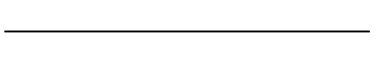
\includegraphics[width=3cm]{bgbacteriano} & $\beta$1,3-Glucano lineal con ramificaciones largas de $\beta$1,6-Glucano\\
Levadura & 
\includegraphics[width=3cm]{bglevadura} & $\beta$1,3-Glucano Lineal \\ 
Cereal & 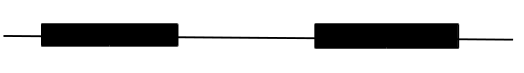
\includegraphics[width=3cm]{bgcereal} & $\beta$1,3/$\beta$1,4-Glucano lineal \\
Hongo & 
\includegraphics[width=3cm]{bghongo} & $\beta$1,3-Glucano lineal con ramificaciones cortas de $\beta$1,6Glucano \\

\bottomrule
\end{tabularx}
\begin{tablenotes}
    \item Estructuras de $\beta$-Glucanos según su origen
\end{tablenotes}
\end{threeparttable}
\end{center}
\end{table}

Los $\beta$-glucanos son carbohidratos que consisten en moléculas de
glucosas enlazadas, los cuales son componentes estructurales de gran
importancia en paredes celulares de levaduras, hongos, algas y algunas
bacterias. Estos carbohidratos también forman parte de la pared celular
endospermas de algunos cereales como la cebada y la avena. Dependiendo
del origen del $\beta$-glucano encontraremos diferencias también en sus
estructuras moleculares y sus posibles ramificaciones (Tabla
\ref{tablaglucanos}) (Skov et al., 2012; Volman et al., 2008).

En peces es ampliamente demostrado el uso de beta-glucanos como
inmunoestimulantes, en distintas especies, como en ciprinidos
(\emph{Cyprinus koi, Cyprinus carpio}) (Kühlwein et al., 2014; S. Lin et
al., 2011)⁠, salmónidos (Abarca, 2011; Skov et al., 2012)⁠, pez cebra
(\emph{Danio rerio}) (Rodríguez et al., 2009), entre otros (Lokesh et
al., 2012; W.-S. Wang et al., 2007), pero como se mencionó anteriormente
todavía existe, a pesar de los antecedentes científicos, cierta
desconfianza en estos inmunoestimulantes.

Dado que las branquias de los peces estan constantemente siendo
``lavadas'' con agua, la cual puede contener patógenos, solo están
cubiertas con una fina capa de mucus, y están construidas de modo que
solo una simple capa de fragiles celulas separa el sistema vascular del
pez del ambiente externo, es muy probable que sean un sitio importante
en la entrada de patógenos. Es mas, las celulas epiteliales de las
branquias son capaces tomar distintas particulas como por ejemplo
esferas de latex (Smith et al 1982) e incluso microorganismos como virus
u otros patógenos.

\clearpage

\section{Hipótesis}\label{hipuxf3tesis}

La administración oral del $\beta$-glucano zimosán en \emph{O.mykiss}
genera una respuesta inmune cuantificable en tejido branquial lo que
permite establecer un modelo de la expresión de moléculas reguladoras y
efectoras de la inmunidad.

\section{Objetivo General}\label{objetivo-general}

Establecer un modelo molecular basado en la cuantificación de diferentes
parámetros de respuesta inmunológica expresada en tejido branquial
\emph{O.mykiss} y relacionada con la administración oral del
$\beta$-glucano zimosán.

\subsection{Objetivos Específicos}\label{objetivos-especuxedficos}

\begin{itemize}
\itemsep1pt\parskip0pt\parsep0pt
\item
  Implementar un sistema de alimentación que permita realizar la
  administración oral de zimosán y sus respectivos controles a O.mykiss
\item
  Evaluar la expresión de moléculas efectoras y reguladoras de respuesta
  inmune en tejido branquial de \emph{O.mykiss} tratados con zimosán vía
  oral
\item
  Detectar la disponibilidad de proteínas efectoras y reguladoras de
  respuesta inmune en tejido branquial de \emph{O.mykiss} tratados con
  zimosán vía oral
\item
  Relacionar el nivel de expresión y detección de moléculas de respuesta
  inmune evaluadas en tejido branquial con el nivel de dosificación oral
  de zimosán.
\end{itemize}

\clearpage

\section{Materiales y Métodos}\label{materiales-y-muxe9todos}

\begin{figure}[h!]
    \centering
        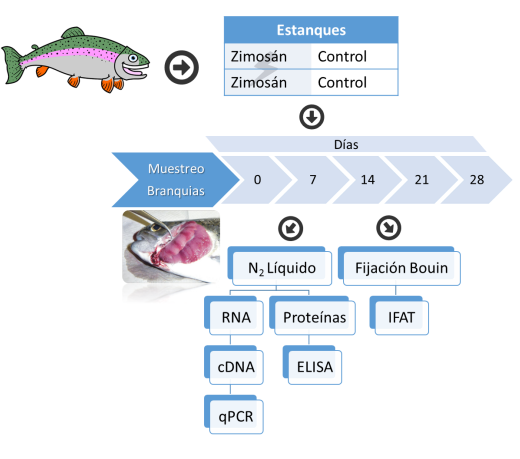
\includegraphics[width=9cm]{esquema} 
    \caption {Esquema general de trabajo}
    \label {fig:esquema}
\end{figure}

\subsection{Material Biológico}\label{material-bioluxf3gico}

\subsubsection{Peces}\label{peces}

Ejemplares de truchas de aproximadamente x meses de edad, con un peso
promedio de 22,26 $\pm$ 1,7397g fueron obtenidas desde la piscicultura
de Rio Blanco, ubicada a 35km de Los Andes, en la Quinta región de
Valparaíso y fueron trasladados hasta el Centro de Investigaciones en
Acuicultura Curauma, ubicado en la provincia de Valparaíso. Fueron
aclimatados durante 1 semana y se mantuvieron a 14º C durante toda la
investigación.

\subsubsection{Anticuerpos}\label{anticuerpos}

Se utilizarán anticuerpos policlonales monoespecíficos, obtenidos en
ratones y conejos, inmunizados con epítopes sintéticos de las moléculas
de interés. Estas moléculas han sido validadas en salmónidos, mediante
técnicas estandarizadas en el Grupo de Marcadores Inmunológicos del
Laboratorio de Genética e Inmunología Molecular de la Pontificia
Universidad Católica de Valparaíso (GIM-PUCV) (J. Bethke et al., 2012;
Narváez et al., 2010; V. Rojas et al., 2012; Santana et al., 2012)

\subsection{Desafío y Controles}\label{desafuxedo-y-controles}

Los especímenes de trucha arcoíris se alimentaran en dos grupos,
inducidos y controles, el primer grupo tendrá una dieta al 3\% de su
peso con un agregado del 0,3\% de Zimosán, los controles tendrán la
misma alimentación excepto por el Zimosán, el cual será reemplazado con
PBS.

\subsection{Muestreo}\label{muestreo}

Los peces se sacrificaron con sobredosis del sedante Kalmagin 20\%
(Benzocaína 20\% ) de CENTROVET, Se tomaron muestras los días 0, 7, 14,
21 y 28, 5 peces por condición, intercalando 3 peces de un estanque y 2
de su par respectivo en cada día de muestreo. Las muestras se tomaron en
dos grupos, primero se tomaron ejemplares de branquias y se fijaron con
solución de Bouin (71\% solución saturada al 1,2\% de Ácido pícrico,
24\% formaldehido y 5\% ácido acético glacial) por 7 horas y luego se
lavaron 3 veces con Etanol al 70\% , dejándolos en este alcohol hasta su
posterior uso. Para el otro grupo se procedió a pulverizar con Nitrogeno
Líquido usando un mortero, para ser usado en las extracciones de RNA y
Proteínas.

\begin{table}[h!]
\sffamily
\begin{center}
    \begin{threeparttable}
    \captionsetup{font={normalsize,sf}}
      \caption{Tabla de identificantes}\label{tablaidentificantes}
      \begin{tabular}{l l l l l l}
    \toprule
    \textbf{ID} & \textbf{Muestra} & \textbf{ID} & \textbf{Muestra} & \textbf{ID} & \textbf{Muestra}\\
    \midrule
    B1 & d0B1 & B26 & d14Bc1 & B41 & d21Bz3 \\
    B2 & d0B2 & B27 & d14Bc1 & B42 & d21Bz3 \\
    B3 & d0B3 & B28 & d14Bc2 & B43 & d21Bz3 \\
    B4 & d0B4 & B29 & d14Bc2 & B44 & d21Bz4 \\
    B5 & d0B5 & B30 & d14Bc2 & B45 & d21Bz4 \\
    B16 & d7Bc1 & B31 & d14Bz3 & B46 & d28Bc1 \\
    B17 & d7Bc1 & B32 & d14Bz3 & B47 & d28Bc1 \\
    B18 & d7Bc1 & B33 & d14Bz4 & B48 & d28Bc2 \\
    B19 & d7Bc2 & B34 & d14Bz4 & B49 & d28Bc2 \\
    B20 & d7Bc2 & B35 & d14Bz4 & B50 & d28Bc2 \\
    B21 & d7Bz3 & B36 & d21Bc1 & B51 & d28Bz3 \\
    B22 & d7Bz3 & B37 & d21Bc1 & B52 & d28Bz3 \\
    B23 & d7Bz3 & B38 & d21Bc1 & B53 & d28Bz4 \\
    B24 & d7Bz4 & B39 & d21Bc2 & B54 & d28Bz4 \\
    B25 & d7Bz4 & B40 & d21Bc2 & B55 & d28Bz4 \\
\bottomrule
\end{tabular}
\begin{tablenotes}
  \item d = Día Muestreo (0,7,14,21,28); B = Branquia; \\
  c = Estanque control (1,2); z = Estanques inducidos (3,4)
\end{tablenotes}
\end{threeparttable}
\end{center}
\end{table}

\clearpage

\subsection{Extracción de RNA}\label{extracciuxf3n-de-rna}

La extracción de RNA se llevó acabo usando el Kit de OmegaBiotek E.Z.N.A
Total RNA Kit II usando las instrucciones del fabricante, para el
homogenizado adicional se usó el homogenizador de sobremesa FastPrep24
de MP Biomedicals con un programa de 4,5 movimientos por segundo durante
40 segundos usando como matriz 4 esferas metálicas de 2,388mm de
diametro.

\subsubsection{Cuantificación e Integridad de
RNA}\label{cuantificaciuxf3n-e-integridad-de-rna}

El RNA se cuantificó usando el sistema espectrofotométrico ND-1000 de
NanoDrop cargando 2uL del RNA previamente extraído, luego para verificar
su integridad se corrió un gel de agarosa nativo al 0,8\% durante 1 hora
a 80V cargando 1$\mu$g de RNA por pocillo, el RNA se almacenó a -80ºC.

\subsubsection{Sintesis de cDNA}\label{sintesis-de-cdna}

La transcripción reversa para generar el DNA complementario al RNA
previamente extraido se realizó usando el Kit M-MLV Reverse
Transcriptase de Promega usando las instrucciones del fabricante con 1µg
de RNA, la reacción se hizo en un Termociclador C1000 Touch de Bio-Rad.

\subsection{PCR en Tiempo Real (qPCR)}\label{pcr-en-tiempo-real-qpcr}

Para todas las reacciones de qPCR se utilizaron el Kit Brilliant III
Ultra-Fast SYBR Green qPCR Master Mix de Agilent Technologies y el
sistema de detección para PCR en Tiempo Real de Bio-Rad CFX96.

\begin{table}[h!]
\sffamily
\begin{center}
%\sffamily
\begin{threeparttable}
%\captionsetup{font={normalsize,sf}}
\caption{Preparación de Master Mix para qPCR}\label{mmix}
\begin{tabularx}{13cm}{X l}
\toprule
 & 1 Reacción \\
\midrule
Brilliant III Ultra-Fast SYBR Green MM & 5$\mu$L \\
Partidores (F+R) 1,5$\mu$M & 4$\mu$L \\
Muestra (1:4) & 1$\mu$L \\
\textbf{Total por reacción} & 10mL \\
\bottomrule
\end{tabularx}
\begin{tablenotes}
    \item Tabla de reactivos para 1 reacción de qPCR
\end{tablenotes}
\end{threeparttable}
\end{center}
\end{table}

\subsubsection{Partidores}\label{partidores}

\begin{table}[h!]
\sffamily
  \begin{center}
    \begin{threeparttable}
      \caption{Lista de Partidores}
      \begin{tabularx}{15cm}{l l X l l}
    \toprule
    Molécula & Partidor & Secuencia & Amplicón & Tm \\
    \midrule
    EF-1$\alpha$ & Fw & \texttt{TGGAGACTGGCACCCTGAAG} & & 58 \\
        & Rev & \texttt{CCAACATTGTCACCAGGCATGG} & & 58 \\
    \midrule
    IL-1$\beta$ & Fw & \texttt{GTCACATTGCCAACCTCATCATCG} & & \\
     & Rev & \texttt{GTTGAGCAGGTCCTTGTCCTTGA} & & \\
     \midrule
     TNF-$\alpha$ & Fw & \texttt{GTGTGGGGTCCTCTTAATAGCAGG} & &  \\
     & Rev & \texttt{CTGCATCGTTGACGGTCTTCC} & &  \\
     \midrule
     IFN-$\gamma$ & Fw & \texttt{GCTGTTCAACGGAAAACCTGTTT} & & \\
      & Rev & \texttt{TCACTGTCCTCAAACGTG} & & \\
     \midrule
     iNOS & Fw & \texttt{TATGCTCTGCCTGCCGTGTC} & & \\
      & Rev & \texttt{ATCCTGCGACCCACTTCCTC} & & \\
     \midrule
     IL-12 & Fw & & & \\
       & Rev & & & \\
\bottomrule
\end{tabularx}
\begin{tablenotes}
    \item Partidores utilizados para la amplificación de los genes en estudio.
\end{tablenotes}
\end{threeparttable}
\end{center}
\end{table}

\subsubsection{Estandarización de
partidores}\label{estandarizaciuxf3n-de-partidores}

Los partidores se estandarizaron con un mix de varios cDNA en distintas
diluciones y usando distintos gradientes dependiendo del partidor,
seleccionando la mejor temperatura en base a su curva patrón y de
fusión.

\begin{table}[h!]
\sffamily
  \begin{center}
    \begin{threeparttable}
      \caption{Programa Termociclador}
      \begin{tabularx}{13cm}{l X l l}
    \toprule
    \textbf{Etapa} & \textbf{Temperatura} & \textbf{Tiempo} & \textbf{Ciclos} \\
    \midrule
    Denaturación Inicial & 95º & 03:00 min & 1 \\
    Denaturación & 95º & 00:10 seg & 39\\
    Annealing en Gradiente & 62º $\rightarrow$ 52$º\textsuperscript{$\dagger$}$ & 00:10 seg & 39 \\
    Extensión & 60º & 00:10 seg & 39 \\
\bottomrule
\end{tabularx}
\begin{tablenotes}
  \item Programa termociclador usado para la estandarización de partidores. 
  $\dagger$\emph{El gradiente varía dentro de esas temperaturas según los partidores}
\end{tablenotes}
\end{threeparttable}
\end{center}
\end{table}

\clearpage

\subsection{Extracción de
Proteínas}\label{extracciuxf3n-de-proteuxednas}

Se agregó una pequeña cantidad de tejido pulverizado a 500$\mu$L de
Buffer de Lisis (Tabla \ref{tablabufferlisis}) y se homogenizó con el
equipo FastPrep24 con un programa de 4,5 movimientos por segundo durante
30 segundos usando como matriz 8 esferas de óxido de zirconio, luego se
dejaron las muestras en hielo durante 30 minutos para posteriormente
centrifugar a máxima velocidad por 5 minutos a 4ºC, se descartó el
precipitado y el sobrenadante se almacenó a -80ºC hasta su uso.

\begin{table}[h!]
\sffamily
  \begin{center}
    \begin{threeparttable}
      \caption{Composición Buffer de Lisis}\label{tablabufferlisis}
      \begin{tabularx}{10cm}{X l}
    \toprule
    \textbf{Compuesto} & \textbf{Concentración} \\
    \midrule
    Tris pH: 7,5 & 0,02M \\
    NaCl & 0,1M \\
    Tritón X-100 & 0,05\% \\
    PMSF & 5mM \\
    \emph{Cocktail} Inhibidor de Proteasas* & 0,2\% \\
\bottomrule
\end{tabularx}
\begin{tablenotes}
  \item *\emph{Sigma Aldrich, P8340}
\end{tablenotes}
\end{threeparttable}
\end{center}
\end{table}

\subsubsection{Cuantificación de
Proteínas}\label{cuantificaciuxf3n-de-proteuxednas}

Para cuantificar las proteínas totales extraídas se usó el método del
ácido bicinconínico (BCA, por sus siglas en inglés), el cual está basado
en la capacidad de este compuesto por formar un intenso complejo purpura
con el ion cuproso en un entorno básico, el cual se produce al
reaccionar las proteínas con cobre alcalino (método Biuret), y el BCA de
cierta forma va censando esta formación (Smith et al., 1985). Se
utilizará el Kit BCA (Pierce), como curva de calibrado se usó albumina
de suero bovino (BSA, por sus siglas en inglés) en diferentes
concentraciones (1,5; 1,0; 0,75; 0,5; 0,25; 0,125 y 0,0125
$\mu$g/$\mu$L) y se leyeron en un lector espectrofotométrico de
microplacas (VersaMax Microplate Reader, Molecular Devices) a 562nm.

\clearpage

\section*{Bibliografía}\label{bibliografuxeda}
\addcontentsline{toc}{section}{Bibliografía}

Abarca, A. (2011). \emph{Implementación de un modelo in vitro para
determinar el poder inmunoestimulante de b-glucanos en macrofagos de
trucha arcoiris} (PhD thesis). Pontificia Universidad Catolica de
Valparaiso.

Abarca, A., Bethke, J., Narváez, E., Flores, R., \& Mercado, L. (2012).
Parameters to evaluate the immunostimulant effect of Zymosan A in head
kidney leucocytes ( HKL ) of salmonids Parámetros para la evaluación del
efecto de Zimosán A como inmunoestimulante sobre leucocitos de riñón
cefálico ( HKL ) de salmónidos, \emph{40}(3), 545--552.

Aghaallaei, N., Bajoghli, B., Schwarz, H., Schorpp, M., \& Boehm, T.
(2010). Characterization of mononuclear phagocytic cells in medaka fish
transgenic for a cxcr3a:gfp reporter. \emph{Proc. Natl. Acad. Sci. U. S.
A.}, \emph{107}(42), 18079--84.

Ainsworth, A. (1992). Fish granulocytes: Morphology, distribution, and
function. \emph{Annu. Rev. Fish Dis.}, \emph{2}, 123--148.

Alvarez-Pellitero, P. (2008). Fish immunity and parasite infections:
from innate immunity to immunoprophylactic prospects. \emph{Vet.
Immunol. Immunopathol.}, \emph{126}(3-4), 171--98.

Athman, R., \& Philpott, D. (2004). Innate immunity via Toll-like
receptors and Nod proteins. \emph{Curr. Opin. Microbiol.}, \emph{7}(1),
25--32.

Bengtén, E., Quiniou, S. M.-A., Stuge, T. B., Katagiri, T., Miller, N.
W., Clem, L. W., \ldots{} Wilson, M. (2002). The IgH Locus of the
Channel Catfish, Ictalurus punctatus, Contains Multiple Constant Region
Gene Sequences: Different Genes Encode Heavy Chains of Membrane and
Secreted IgD. \emph{J. Immunol.}, \emph{169}(5), 2488--2497.

Bethke, J., Rojas, V., Berendsen, J., Cárdenas, C., Guzmán, F.,
Gallardo, J. A., \& Mercado, L. (2012). Development of a new antibody
for detecting natural killer enhancing factor (NKEF)-like protein in
infected salmonids. \emph{J. Fish Dis.}, \emph{35}(5), 379--88.

Bilen, S., Bulut, M., \& Bilen, A. M. (2011). Immunostimulant effects of
Cotinus coggyria on rainbow trout (Oncorhynchus mykiss). \emph{Fish
Shellfish Immunol.}, \emph{30}(2), 451--5.

Boehm, U., Klamp, T., Groot, M., \& Howard, J. C. (1997). Cellular
responses to interferon-gamma. \emph{Annu. Rev. Immunol.}, \emph{15},
749--95.

Bogdan, C. (2001). Nitric oxide and the immune response. \emph{Nat.
Immunol.}, \emph{2}(10), 907--16.

Bols, N. C., Brubacher, J. L., Ganassin, R. C., \& Lee, L. E. (2001).
Ecotoxicology and innate immunity in fish. \emph{Dev. Comp. Immunol.},
\emph{25}(8-9), 853--873.

Bricknell, I., \& Dalmo, R. a. (2005). The use of immunostimulants in
fish larval aquaculture. \emph{Fish Shellfish Immunol.}, \emph{19}(5),
457--72.

Castro, R., Bernard, D., Lefranc, M. P., Six, a, Benmansour, a, \&
Boudinot, P. (2011). T cell diversity and TcR repertoires in teleost
fish. \emph{Fish Shellfish Immunol.}, \emph{31}(5), 644--54.

Chang, C.-i., Pleguezuelos, O., Zhang, Y.-a., Zou, J., \& Secombes, C.
J. (2005). Identification of a novel cathelicidin gene in the rainbow
trout, Oncorhynchus mykiss. \emph{Infect. Immun.}, \emph{73}(8),
5053--64.

Chang, C.-I., Zhang, Y.-A., Zou, J., Nie, P., \& Secombes, C. J. (2006).
Two cathelicidin genes are present in both rainbow trout (Oncorhynchus
mykiss) and atlantic salmon (Salmo salar). \emph{Antimicrob. Agents
Chemother.}, \emph{50}(1), 185--95.

Chettri, J. K., Kania, P. W., \& Buchmann, K. (2013). Immunomodulation
of rainbow trout ( Oncorhynchus mykiss ) fry by bath exposure to a
$\beta$-glucan from Euglena gracilis. \emph{Aquac. Res.}, \emph{44}(9),
1407--1415.

Dalmo, R. a, \& Bøgwald, J. (2008). Beta-glucans as conductors of immune
symphonies. \emph{Fish Shellfish Immunol.}, \emph{25}(4), 384--96.

Ellis, A. E. (1977). The leucocytes of fish: A review. \emph{J. Fish
Biol.}, \emph{11}(5), 453--491.

Ellis, A. E. (2001). Innate host defense mechanisms of fish against
viruses and bacteria. \emph{Dev. Comp. Immunol.}, \emph{25}(8-9),
827--39.

FAO. (2012). \emph{El estado mundial de la pesca y la acuicultura -
2012} (p. 251).

Fernández, A., Ruiz, I., \& Blas, I. D. (2002). El sistema inmune de los
teleósteos (I): Células y órganos. \emph{Rev. Aquat.}, \emph{16}.

Fields, B. N., Knipe, D. M., \& Howley, P. M. (2007). \emph{Fields'
Virology}. Wolters Kluwer Health/Lippincott Williams \& Wilkins.

Georgiadis, M., Gardner, I., \& Hedrick, R. (2001). The role of
epidemiology in the prevention, diagnosis, and control of infectious
diseases of fish. \emph{Prev. Vet. Med.}, \emph{48}(4), 287--302.

Gordon, S. (2002). Pattern recognition receptors: doubling up for the
innate immune response. \emph{Cell}, \emph{111}(7), 927--30.

Graves, S. S., Evans, D. L., Cobb, D., \& Dawe, D. L. (1984).
Nonspecific cytotoxic cells in fish (Ictalurus punctatus). I. Optimum
requirements for target cell lysis. \emph{Dev. Comp. Immunol.},
\emph{8}(2), 293--302.

Groot, C., \& Margolis, L. (1991). \emph{Pacific Salmon Life Histories}.
University of British Columbia Press.

Hong, S., Zou, J., Collet, B., Bols, N. C., \& Secombes, C. J. (2004).
Analysis and characterisation of IL-1beta processing in rainbow trout,
Oncorhynchus mykiss. \emph{Fish Shellfish Immunol.}, \emph{16}(3),
453--9.

Huising, M. O., Schijndel, J. E. van, Kruiswijk, C. P., Nabuurs, S. B.,
Savelkoul, H. F. J., Flik, G., \& {Verburg-van Kemenade}, B. M. L.
(2006). The presence of multiple and differentially regulated
interleukin-12p40 genes in bony fishes signifies an expansion of the
vertebrate heterodimeric cytokine family. \emph{Mol. Immunol.},
\emph{43}(10), 1519--33.

Kawai, T., \& Akira, S. (2005). Pathogen recognition with Toll-like
receptors. \emph{Curr. Opin. Immunol.}, \emph{17}(4), 338--44.

Kumari, J., \& Sahoo, P. K. (2006). Dietary immunostimulants influence
specific immune response and resistance of healthy and immunocompromised
Asian catfish Clarias batrachus to Aeromonas hydrophila infection.
\emph{Dis. Aquat. Organ.}, \emph{70}(1-2), 63--70.

Kühlwein, H., Merrifield, D. L., Rawling, M. D., Foey, a D., \& Davies,
S. J. (2014). Effects of dietary $\beta$-(1,3)(1,6)-D-glucan
supplementation on growth performance, intestinal morphology and
haemato-immunological profile of mirror carp (Cyprinus carpio L.).
\emph{J. Anim. Physiol. Anim. Nutr. (Berl).}, \emph{98}(2), 279--89.

Lin, S., Pan, Y., Luo, L., \& Luo, L. (2011). Effects of dietary
$\beta$-1,3-glucan, chitosan or raffinose on the growth, innate immunity
and resistance of koi (Cyprinus carpio koi). \emph{Fish Shellfish
Immunol.}, \emph{31}(6), 788--94.

Lokesh, J., Fernandes, J. M. O., Korsnes, K., Bergh, O., Brinchmann, M.
F., \& Kiron, V. (2012). Transcriptional regulation of cytokines in the
intestine of Atlantic cod fed yeast derived mannan oligosaccharide or
$\beta$-glucan and challenged with Vibrio anguillarum. \emph{Fish
Shellfish Immunol.}, \emph{33}(3), 626--31.

MacMicking, J., Xie, Q. W., \& Nathan, C. (1997). Nitric oxide and
macrophage function. \emph{Annu. Rev. Immunol.}, \emph{15}, 323--50.

Maier, V. H., Dorn, K. V., Gudmundsdottir, B. K., \& Gudmundsson, G. H.
(2008). Characterisation of cathelicidin gene family members in
divergent fish species. \emph{Mol. Immunol.}, \emph{45}(14), 3723--30.

Mercado, L., Schmitt, P., Marshall, S. H., \& Arenas, G. (2005). Gill
tissues of the mussel Mytilus edulis chilensis: A new source for
antimicrobial peptides. \emph{Electron. J. Biotechnol.}, \emph{8}(3),
284--290.

Narváez, E., Berendsen, J., Guzmán, F., Gallardo, J. a, \& Mercado, L.
(2010). An immunological method for quantifying antibacterial activity
in Salmo salar (Linnaeus, 1758) skin mucus. \emph{Fish Shellfish
Immunol.}, \emph{28}(1), 235--9.

Nascimento, D. S., Vale, A. do, Tomás, A. M., Zou, J., Secombes, C. J.,
\& Santos, N. M. S. dos. (2007). Cloning, promoter analysis and
expression in response to bacterial exposure of sea bass (Dicentrarchus
labrax L.) interleukin-12 p40 and p35 subunits. \emph{Mol. Immunol.},
\emph{44}(9), 2277--91.

Olabuenaga, S. E. (2000). Sistema inmune en peces. \emph{Gayana
(Concepción)}, \emph{64}(2).

Palić, D., Beck, L. S., Palić, J., \& Andreasen, C. B. (2011). Use of
rapid cytochemical staining to characterize fish blood granulocytes in
species of special concern and determine potential for function testing.
\emph{Fish Shellfish Immunol.}, \emph{30}(2), 646--52.

Peddie, S., Zou, J., \& Secombes, C. J. (2002). Immunostimulation in the
rainbow trout (Oncorhynchus mykiss) following intraperitoneal
administration of Ergosan. \emph{Vet. Immunol. Immunopathol.},
\emph{86}(1-2), 101--113.

Razquin, B. E., Castillo, A., Lopez-Fierro, P., Alvarez, F., Zapata, A.,
\& Villena, A. J. (1990). Ontogeny of IgM-producing cells in the
lymphoid organs of rainbow trout, Salmo gairdneri Richardson: an immuno-
and enzyme-histochemical study. \emph{J. Fish Biol.}, \emph{36}(2),
159--173.

Reis, M. I. R., Vale, A. do, Pereira, P. J. B., Azevedo, J. E., \& {Dos
Santos}, N. M. S. (2012). Caspase-1 and IL-1$\beta$ processing in a
teleost fish. \emph{PLoS One}, \emph{7}(11), e50450.

Rodríguez, I., Chamorro, R., Novoa, B., \& Figueras, A. (2009).
beta-Glucan administration enhances disease resistance and some innate
immune responses in zebrafish (Danio rerio). \emph{Fish Shellfish
Immunol.}, \emph{27}(2), 369--73.

Rojas, V., Guzman, F., \& Morales-lange, B. (2012). Immunological
strategy for detecting the pro-inflammatory cytokine TNF-alpha in
salmonids. \emph{Electron. J. Biotechnol.}, \emph{15}.

Rondon-Barragan, I. (2010). Receptores similares a Toll en peces : el
inicio de la divergencia. \emph{Investig. Vet.}, \emph{11}(1), 15--30.

Salazar-Mather, T., \& Hokeness, K. (2006). Cytokine and Chemokine
Networks: Pathways to Antiviral Defense. In T. E. Lane (ed.),
\emph{Chemokines Viral Infect.} (Vol. 303, pp. 29--46). Springer Berlin
Heidelberg.

Santana, P., Palacios, C., Narváez, E., \& Guzmán, F. (2012).
Anti-peptide antibodies : A tool for detecting IL-8 in salmonids,
\emph{15}.

Savan, R., \& Sakai, M. (2006). Genomics of fish cytokines. \emph{Comp.
Biochem. Physiol. Part D. Genomics Proteomics}, \emph{1}(1), 89--101.

Secombes, C. J., Wang, T., \& Bird, S. (2011). The interleukins of fish.
\emph{Dev. Comp. Immunol.}, \emph{35}(12), 1336--45.

Sernapesca. (2012). Anuario desembarques. Santiago de Chile: Gobierno de
Chile.

Shao, Z. J. (2001). Aquaculture pharmaceuticals and biologicals: current
perspectives and future possibilities. \emph{Adv. Drug Deliv. Rev.},
\emph{50}(3), 229--243.

Skov, J., Kania, P. W., Holten-Andersen, L., Fouz, B., \& Buchmann, K.
(2012). Immunomodulatory effects of dietary $\beta$-1,3-glucan from
Euglena gracilis in rainbow trout (Oncorhynchus mykiss) immersion
vaccinated against Yersinia ruckeri. \emph{Fish Shellfish Immunol.},
\emph{33}(1), 111--20.

Smith, P. K., Krohn, R. I., Hermanson, G. T., Mallia, A. K., Gartner, F.
H., Provenzano, M. D., \ldots{} Klenk, D. C. (1985). Measurement of
protein using bicinchoninic acid. \emph{Anal. Biochem.}, \emph{150}(1),
76--85.

Subpesca. (2013). Cuenta Pública de Estado de los Recursos. Santiago de
Chile: Gobierno de Chile.

Taechavasonyoo, A., Kondo, H., Nozaki, R., Suzuki, Y., \& Hirono, I.
(2013). Identification of novel interleukin 1 beta family genes in
Japanese flounder Paralichthys olivaceus. \emph{Fish Shellfish
Immunol.}, \emph{34}(1), 393--6.

Teles, M., Mackenzie, S., Boltaña, S., Callol, a, \& Tort, L. (2011).
Gene expression and TNF-alpha secretion profile in rainbow trout
macrophages following exposures to copper and bacterial
lipopolysaccharide. \emph{Fish Shellfish Immunol.}, \emph{30}(1),
340--6.

Volman, J. J., Ramakers, J. D., \& Plat, J. (2008). Dietary modulation
of immune function by beta-glucans. \emph{Physiol. Behav.},
\emph{94}(2), 276--84.

Wang, T., Johnson, N., Zou, J., Bols, N., \& Secombes, C. J. (2004).
Sequencing and expression of the second allele of the interleukin-1beta1
gene in rainbow trout (Oncorhynchus mykiss): identification of a novel
SINE in the third intron. \emph{Fish Shellfish Immunol.}, \emph{16}(3),
335--58.

Wang, W.-S., Hung, S.-W., Lin, Y.-H., Tu, C.-Y., Wong, M.-L., Chiou,
S.-H., \& Shieh, M.-T. (2007). The effects of five different glycans on
innate immune responses by phagocytes of hybrid tilapia and Japanese
eels Anguilla japonica. \emph{J. Aquat. Anim. Health}, \emph{19}(1),
49--59.

Whyte, S. K. (2007). The innate immune response of finfish--a review of
current knowledge. \emph{Fish Shellfish Immunol.}, \emph{23}(6),
1127--51.

Wimley, W. C. (2010). Describing the mechanism of antimicrobial peptide
action with the interfacial activity model. \emph{ACS Chem. Biol.},
\emph{5}(10), 905--17.

Wu, F., Tyml, K., \& Wilson, J. X. (2008). iNOS expression requires
NADPH oxidase-dependent redox signaling in microvascular endothelial
cells. \emph{J. Cell. Physiol.}, \emph{217}(1), 207--14.

Yang, K., Zhang, S., Chen, D., Zhang, A., Wang, X., \& Zhou, H. (2013).
IFN-$\gamma$-activated lymphocytes boost nitric oxide production in
grass carp monocytes/macrophages. \emph{Fish Shellfish Immunol.},
\emph{35}(5), 1635--41.

Yoshiura, Y., Kiryu, I., Fujiwara, A., Suetake, H., Suzuki, Y.,
Nakanishi, T., \& Ototake, M. (2003). Identification and
characterization of Fugu orthologues of mammalian interleukin-12
subunits. \emph{Immunogenetics}, \emph{55}(5), 296--306.

Zasloff, M. (2002). Antimicrobial peptides of multicellular organisms.
\emph{Nature}, \emph{415}(6870), 389--95.

Zhang, L., Li, Y.-y., Chen, T., Xia, W., Zhou, Y., Wan, Y.-j., \ldots{}
Xu, S.-q. (2011). Abnormal development of motor neurons in
perfluorooctane sulphonate exposed zebrafish embryos.
\emph{Ecotoxicology}, \emph{20}(4), 643--52.

Zhang, L., Zhang, B.-C., \& Hu, Y.-H. (2014). Rock bream (Oplegnathus
fasciatus) IL-12p40: identification, expression, and effect on bacterial
infection. \emph{Fish Shellfish Immunol.}

Zhang, Z., Swain, T., Bøgwald, J., Dalmo, R. a, \& Kumari, J. (2009).
Bath immunostimulation of rainbow trout (Oncorhynchus mykiss) fry
induces enhancement of inflammatory cytokine transcripts, while repeated
bath induce no changes. \emph{Fish Shellfish Immunol.}, \emph{26}(5),
677--84.

Zhao, K., Huang, Z., Lu, H., Zhou, J., \& Wei, T. (2010). Induction of
inducible nitric oxide synthase increases the production of reactive
oxygen species in RAW264.7 macrophages. \emph{Biosci. Rep.},
\emph{30}(4), 233--41.

Zhu, L.-Y., Nie, L., Zhu, G., Xiang, L.-X., \& Shao, J.-Z. (2012).
Advances in research of fish immune-relevant genes: A comparative
overview of innate and adaptive immunity in teleosts. \emph{Dev. Comp.
Immunol.}

Zou, J., Peddie, S., Scapigliati, G., Zhang, Y., Bols, N., Ellis, \&
Secombes, C. (2003). Functional characterisation of the recombinant
tumor necrosis factors in rainbow trout, Oncorhynchus mykiss. \emph{Dev.
Comp. Immunol.}, \emph{27}(9), 813--822.

\end{document}
